\begin{figure}[htb]
\centering
\begin{subfigure}{.49\textwidth}
	\centering
        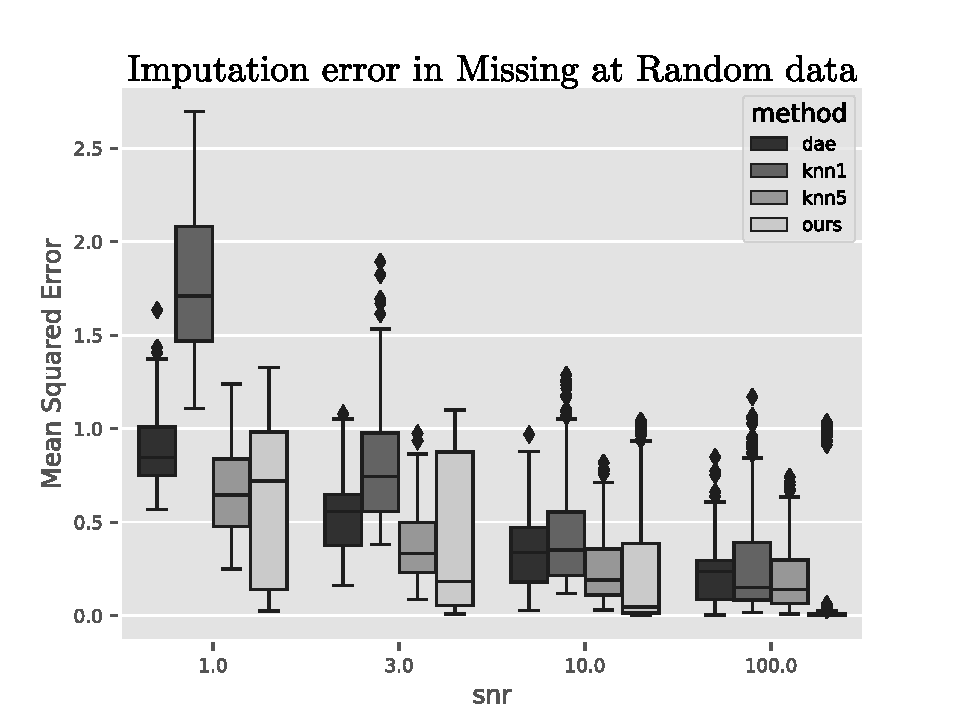
\includegraphics[width=\textwidth]{./tex/fig/mar_imput_err_boxplot.pdf}
        \caption{Missing at random}
        \label{fig:synthetic_benchmark_mar_box}
\end{subfigure}%
\hfill
\begin{subfigure}{.49\textwidth}
	\centering
        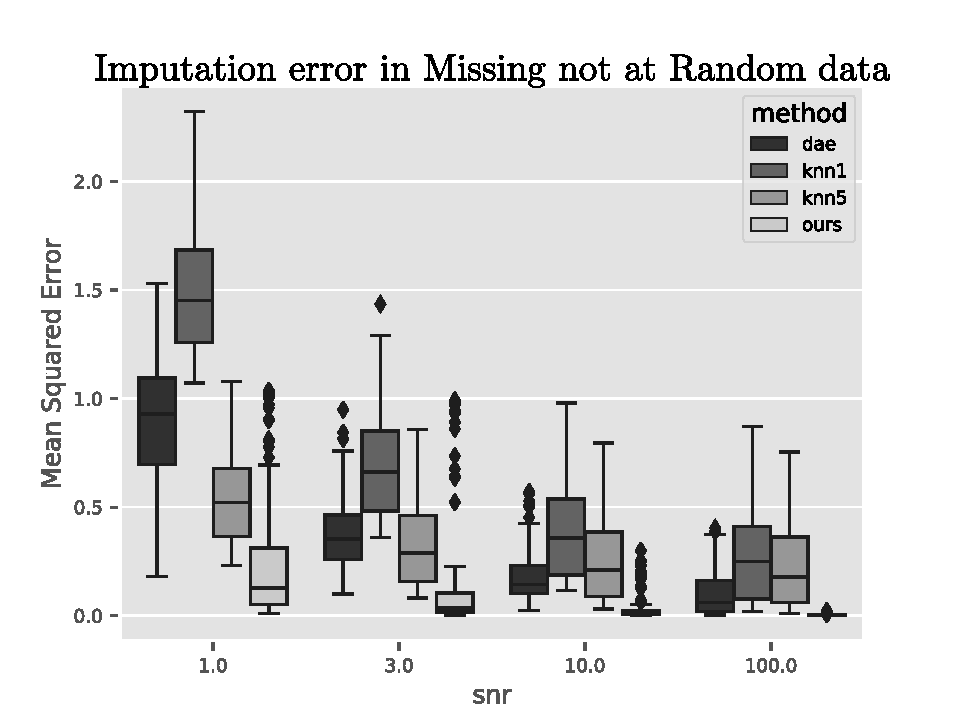
\includegraphics[width=\textwidth]{./tex/fig/mnar_imput_err_boxplot.pdf}
        \caption{Missing not at random}
        \label{fig:synthetic_benchmark_mnar_box}
\end{subfigure}
\caption{
Mean Squared Error (MSE) of imputation in synthetic held-out datasets ($5$-folds cross-validation).
Compared to the best competing methods among $k$-Nearest Neighbor ($k=\set{1, 5}$) and Denoise Autoencoder (DAE), our model comes out as the best performer, with a mean MSE improvement of $17\%$ in MAR cases (a) and $71\%$ in MNAR cases (b).
Stratification by signal-to-noise ratio (\snr) is shown.
}
\label{fig:synthetic_benchmark_box}
\end{figure}

\begin{figure}[htb]
\centering
\begin{subfigure}{.49\textwidth}
	\centering
        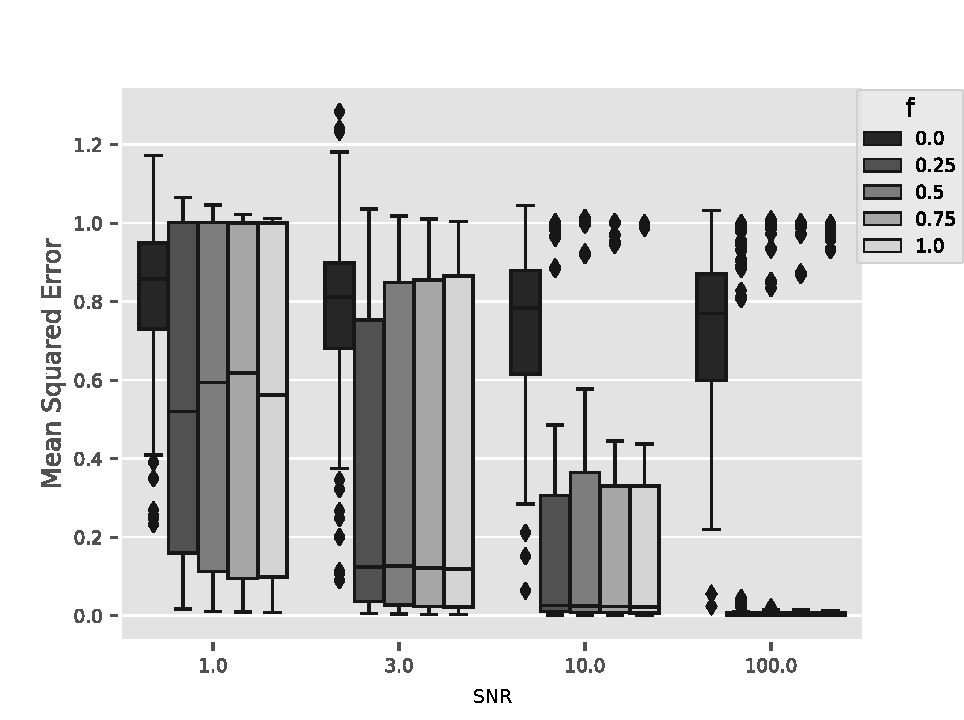
\includegraphics[width=\textwidth]{./tex/fig/mar_pred_err_boxplot.pdf}
        % \caption{Missing at random}
        % \label{fig:synthetic_benchmark_mar_pred_box}
\end{subfigure}%
\caption{
Mean Squared Error of test sets predictions in synthetic hold-out datasets).
We show how with already $f \geq 0.25$ (the fraction of observations with all the views) we can significantly reduce the prediction error on testing data-points.
}
\label{fig:synthetic_benchmark_pred_box}
\end{figure}
% \begin{figure}[htb]
% \centering
% \begin{subfigure}{.45\textwidth}
%       \centering
%         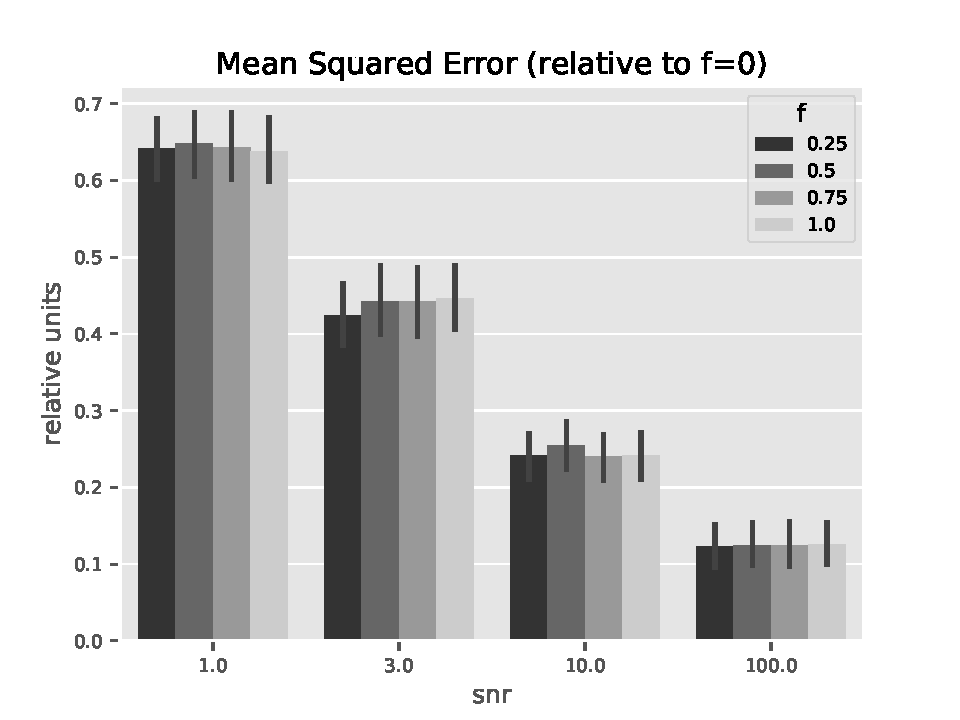
\includegraphics[width=\textwidth]{./tex/fig/mar_barplot.pdf}
%         \caption{Missing at random}
%         \label{fig:synthetic_benchmark_mar_bar}
% \end{subfigure}%
% \hfill
% \begin{subfigure}{.45\textwidth}
%       \centering
%         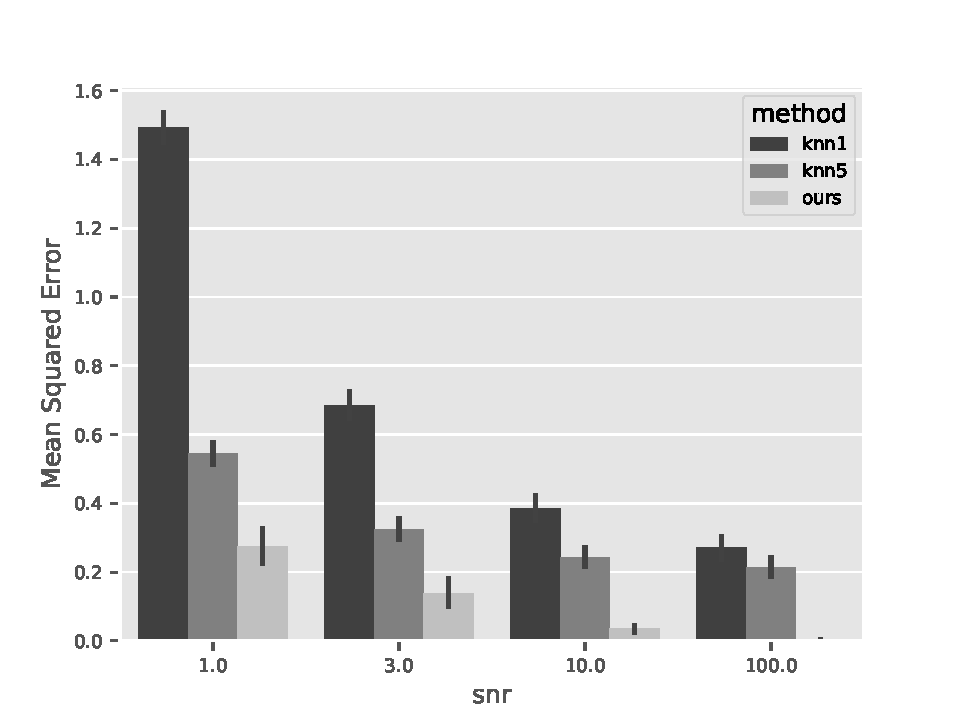
\includegraphics[width=\textwidth]{./tex/fig/mnar_barplot.pdf}
%         \caption{Missing not at random}
%         \label{fig:synthetic_benchmark_mnar_bar}
% \end{subfigure}
% \caption{
% Mean Squared Error of test sets predictions in synthetic datasets. Effect of signal-to-noise ratio (\snr) is shown.
% (a) With $f$ being the fraction of observation with complete views, we show how with already $f \geq 0.25$ we can significantly reduce the prediction error on testing data-points.
% (b) In multi-view datasets where none of the data-point have all the views, and where the available views depends on the specific dataset, we show the prediction performance of our model in comparison with classic k-nearest-neighbors imputation methods.
% }
% \label{fig:synthetic_benchmark_bar}
% \end{figure}

